% Reviewed translation: PDF pages 187--193 / printed pages 173--179.
% The original scan is authoritative; environment headings remain English.

\section{压力的连续逼近}\label{sec:primitive-continuous-pressure}

到目前为止, 所用近似压力在单元界面上(一般而言)是不连续的. 但从工程观点看,
连续压力更为自然, 因为实际遇到的压力通常是连续函数. 事实上, 数值分析工作者发现,
带 $C^0$ 压力的 Stokes 求解器比带 $L^2$ 压力的求解器更难分析. 这一困难解释了
为什么关于重要的“Hood--Taylor”型格式的理论文献相对较少.

对广泛使用的 Hood \& Taylor 格式, 第一个严格的误差分析由
Bercovier \& Pironneau 给出. 后来 Verfürth 巧妙地简化了这一分析;
而现在, Subsection~\ref{subsec:primitive-discrete-inf-sup-methods} 的方法
可把 Hood--Taylor 方法直接纳入 Section~\ref{sec:primitive-general-approximation}
的框架.

除 Hood--Taylor 格式及其密切相关的格式外, 本节还研究
Glowinski \& Pironneau 引入的一个有趣变体, 它用一系列 $-\Delta$ 的离散
Dirichlet 问题逼近 Stokes 问题.

\MathBookSourcePage{188}
\subsection{一阶方法: ``Mini'' 有限元}\label{subsec:primitive-mini-element}

只需稍作修改, 问题的设定与
Subsection~\ref{subsec:primitive-homogeneous-stokes} 相同. 取 $\Omega$ 为有界平面
多边形, 并假设 Stokes 系统
\begin{equation}\label{eq:primitive-continuous-pressure-stokes-system}
\left\{
\begin{aligned}
-\nu\Delta\mathbf u+\operatorname{grad}p&=\mathbf f,
&\operatorname{div}\mathbf u&=0 &&\text{in }\Omega,\\
\mathbf u&=\mathbf0 &&&\text{on }\Gamma
\end{aligned}
\right.
\end{equation}
中的压力满足 $p\in H^1(\Omega)$.

按照 Arnold et al., 构造 $\overline\Omega$ 的三角剖分 $\mathcal T_h$, 并在每个
单元 $\kappa$ 上用下列空间的多项式逼近速度:
\begin{equation}\label{eq:primitive-mini-local-space}
\mathcal P_1(\kappa)
=\bigl[P_1\oplus\operatorname{span}\{\lambda_1\lambda_2\lambda_3\}\bigr]^2,
\end{equation}
而压力用 $P_1$ 中的多项式逼近. 因而选取有限元空间
\begin{equation}\label{eq:primitive-mini-velocity-space}
X_h=\{\mathbf v\in C^0(\overline\Omega)^2;
\ \mathbf v|_\kappa\in\mathcal P_1(\kappa)\ \forall\kappa\in\mathcal T_h,
\ \mathbf v|_\Gamma=\mathbf0\},
\end{equation}
\begin{equation}\label{eq:primitive-continuous-linear-pressure-spaces}
Q_h=\{q\in C^0(\overline\Omega);\ q|_\kappa\in P_1
\ \forall\kappa\in\mathcal T_h\},
\qquad M_h=Q_h\cap L_0^2(\Omega).
\end{equation}
自由度最为简单: 速度在 $\kappa$ 的顶点和中心处的值, 以及压力在
$\kappa$ 的顶点处的值. 与往常一样, 定义
\[
V_h=\{\mathbf v_h\in X_h;
(\operatorname{div}\mathbf v_h,q_h)=0\ \forall q_h\in Q_h\},
\]
并把下列近似问题称为问题 $(Q_h)$: 求
$(\mathbf u_h,p_h)\in X_h\times M_h$, 使
\begin{equation}\label{eq:primitive-continuous-pressure-discrete-problem}
\left\{
\begin{aligned}
a(\mathbf u_h,\mathbf v_h)-(p_h,\operatorname{div}\mathbf v_h)
&=\langle\mathbf f,\mathbf v_h\rangle
&&\forall\mathbf v_h\in X_h,\\
(\operatorname{div}\mathbf u_h,q_h)&=0
&&\forall q_h\in Q_h.
\end{aligned}
\right.
\end{equation}
双线性形式 $a(\cdot,\cdot)$ 保持不变:
\[
a(\mathbf u,\mathbf v)=2\nu\sum_{i,j=1}^2
(D_{ij}(\mathbf u),D_{ij}(\mathbf v)),
\]
或
\[
a(\mathbf u,\mathbf v)=\nu(\operatorname{grad}\mathbf u,
\operatorname{grad}\mathbf v).
\]
注意, 因为空间 $Q_h$ 包含于 $H^1(\Omega)$, 双线性形式
$b(\cdot,\cdot)$ 也可等价地写为
\[
b(\mathbf v_h,q_h)=-(\operatorname{div}\mathbf v_h,q_h)
=(\operatorname{grad}q_h,\mathbf v_h)
\quad\forall\mathbf v_h\in X_h,\ \forall q_h\in Q_h.
\]

\MathBookSourcePage{189}
$X_h$ 与 $Q_h$ 的逼近性质是熟知的. 例如, 若三角剖分 $\mathcal T_h$ 正则,
由
\begin{equation}\label{eq:primitive-mini-interpolant-definition}
\left\{
\begin{aligned}
r_h\mathbf v(a)&=\mathbf v(a)
&&\text{在 }\mathcal T_h\text{ 的所有节点 }a\text{ 上},\\
r_h\mathbf v(a_\kappa)&=\mathbf v(a_\kappa)
&&\text{在每个 }\kappa\in\mathcal T_h\text{ 的中心 }a_\kappa\text{ 上},\\
r_h\mathbf v&\in\mathcal P_1(\kappa)
&&\text{在每个 }\kappa\text{ 上}
\end{aligned}
\right.
\end{equation}
定义的插值算子 $r_h$ 满足
\[
r_h\in\mathcal L([H^2(\Omega)\cap H_0^1(\Omega)]^2;X_h),
\]
以及
\begin{equation}\label{eq:primitive-mini-interpolation-error}
\|\mathbf v-r_h\mathbf v\|_{m,\Omega}
\leq Ch^{2-m}|\mathbf v|_{2,\Omega}
\quad\forall\mathbf v\in H^2(\Omega)^2,
\quad m=0\text{ 或 }1.
\end{equation}
事实上, $r_h$ 在每个 $\kappa$ 上被仿射变换保持, 并保持 $P_1^2$ 中的多项式不变.

类似地, 由 \eqref{eq:appendix-local-regularization-projection} 和
\eqref{eq:appendix-local-regularization-interpolant} 定义的 $P_1$ 上局部正则化算子
$R_h$ 满足 $R_h\in\mathcal L(L^2(\Omega);Q_h)$, 且
\begin{equation}\label{eq:primitive-continuous-pressure-regularization-error}
\|q-R_hq\|_{m,\Omega}
\leq Ch^{1-m}|q|_{1,\Omega}
\quad\forall q\in H^1(\Omega),
\quad m=0\text{ 或 }1,
\end{equation}
当然这里要求 $\mathcal T_h$ 正则.

因此 Hypotheses H1 和 H2 成立, 只需验证 H3, 即 inf-sup 条件
\begin{equation}\label{eq:primitive-continuous-pressure-inf-sup}
\sup_{\mathbf v_h\in X_h}
\frac{(q_h,\operatorname{div}\mathbf v_h)}{|\mathbf v_h|_{1,\Omega}}
\geq\beta^*\|q_h\|_{0,\Omega}
\qquad\forall q_h\in M_h.
\end{equation}
这由下一个 Lemma 完成.

\setcounter{statement}{0}
\renewcommand{\theHstatement}{lemma.\thesection.\arabic{statement}}
\begin{Lemma}\label{lem:primitive-mini-inf-sup}
若三角剖分 $\mathcal T_h$ 正则, 则由
\eqref{eq:primitive-mini-velocity-space} 和
\eqref{eq:primitive-continuous-linear-pressure-spaces} 定义的空间对
$(X_h,M_h)$ 满足 \eqref{eq:primitive-continuous-pressure-inf-sup},
其中常数 $\beta^*>0$ 与 $h$ 无关.
\end{Lemma}

\begin{Proof}
构造 Lemma~\ref{lem:primitive-fortin-criterion} 中的算子 $\pi_h$.
任取 $q_h\in M_h$. 因为 $q_h\in L_0^2(\Omega)$, 存在
$\mathbf v\in H_0^1(\Omega)^2$ 使
\begin{equation}\label{eq:primitive-mini-divergence-lifting}
\operatorname{div}\mathbf v=q_h,
\qquad |\mathbf v|_{1,\Omega}\leq C_1\|q_h\|_{0,\Omega}.
\end{equation}
因此, 由于 $M_h\subset H^1(\Omega)$, 我们要构造
$\pi_h\mathbf v\in X_h$ 使
\[
\sum_{\kappa\in\mathcal T_h}\int_\kappa
\pi_h\mathbf v\cdot\operatorname{grad}\mu_h\,dx
=\sum_{\kappa\in\mathcal T_h}\int_\kappa
\mathbf v\cdot\operatorname{grad}\mu_h\,dx
\qquad\forall\mu_h\in M_h.
\]
因为每个 $\kappa$ 上 $\operatorname{grad}\mu_h\in P_0^2$, 这提示按下式定义
$\pi_h\mathbf v\in X_h$:
\begin{equation}\label{eq:primitive-mini-fortin-nodal-values}
\pi_h\mathbf v(a)=(R_h\mathbf v)(a)
\qquad\forall\mathcal T_h\text{ 的节点 }a,
\end{equation}
以及
\MathBookSourcePage{190}
\begin{equation}\label{eq:primitive-mini-fortin-cell-moments}
\int_\kappa\pi_h\mathbf v\,dx
=\int_\kappa\mathbf v\,dx
\qquad\forall\kappa\in\mathcal T_h,
\end{equation}
其中 $R_h$ 表示现在已经熟悉的 $P_1^2$ 上局部正则化算子.

显然, \eqref{eq:primitive-mini-fortin-nodal-values} 和
\eqref{eq:primitive-mini-fortin-cell-moments} 唯一确定 $X_h$ 中的
$\pi_h\mathbf v$, 且
$\pi_h\in\mathcal L(H_0^1(\Omega)^2;X_h)$. 此外
\[
\int_\Omega\operatorname{div}(\pi_h\mathbf v-\mathbf v)\mu_h\,dx=0
\qquad\forall\mu_h\in M_h.
\]
最后, 与 Lemma~\ref{lem:primitive-bernardi-raugel-fortin-estimates}
类似的论证表明, 若 $\mathcal T_h$ 正则, 则
\[
|\pi_h\mathbf v|_{1,\Omega}\leq C_2|\mathbf v|_{1,\Omega}.
\]
这就证明了 Lemma.
\end{Proof}

这些结果汇总为下列 Theorem.

\setcounter{statement}{0}
\renewcommand{\theHstatement}{theorem.\thesection.\arabic{statement}}
\begin{Theorem}\label{thm:primitive-mini-error}
设 $\Omega$ 是有界平面多边形, 且 Stokes 系统
\eqref{eq:primitive-continuous-pressure-stokes-system} 的解 $(\mathbf u,p)$ 满足
\[
\mathbf u\in[H^2(\Omega)\cap H_0^1(\Omega)]^2,
\qquad p\in H^1(\Omega)\cap L_0^2(\Omega).
\]
若三角剖分 $\mathcal T_h$ 正则, 则使用分别由
\eqref{eq:primitive-mini-velocity-space} 和
\eqref{eq:primitive-continuous-linear-pressure-spaces} 定义的空间 $X_h,M_h$ 时,
问题 \eqref{eq:primitive-continuous-pressure-discrete-problem} 的解
$(\mathbf u_h,p_h)$ 满足误差界
\begin{equation}\label{eq:primitive-mini-h1-pressure-error}
|\mathbf u-\mathbf u_h|_{1,\Omega}+\|p-p_h\|_{0,\Omega}
\leq C_1h\{\|\mathbf u\|_{2,\Omega}+|p|_{1,\Omega}\}.
\end{equation}
此外, 当 $\Omega$ 为凸集时, 有 $L^2$ 估计
\begin{equation}\label{eq:primitive-mini-l2-error}
\|\mathbf u-\mathbf u_h\|_{0,\Omega}
\leq C_2h^2\{\|\mathbf u\|_{2,\Omega}+|p|_{1,\Omega}\}.
\end{equation}
\end{Theorem}

这种“mini”有限元方法很容易推广到任意阶格式. 细节可见 Arnold et al.

\subsection{``Hood--Taylor'' 有限元方法}\label{subsec:primitive-hood-taylor}

采用更精确的速度逼近可以改进上一小节的结果. 按照 Hood \& Taylor,
保留同一空间 $Q_h$, 并把 $X_h$ 替换为
\begin{equation}\label{eq:primitive-hood-taylor-velocity-space}
X_h=\{\mathbf v\in C^0(\overline\Omega)^2;
\ \mathbf v|_\kappa\in P_2^2\ \forall\kappa\in\mathcal T_h,
\ \mathbf v|_\Gamma=\mathbf0\},
\end{equation}
其自由度取为二阶主格点(参见
\eqref{eq:appendix-lagrange-interpolant-definition})上的函数值. 因此标准插值算子
$I_h$ 满足
\[
I_h\in\mathcal L([H^k(\Omega)\cap H_0^1(\Omega)]^2;X_h),
\]
以及
\begin{equation}\label{eq:primitive-hood-taylor-interpolation-error}
\|\mathbf v-I_h\mathbf v\|_{m,\Omega}
\leq Ch^{k-m}|\mathbf v|_{k,\Omega}
\quad\forall\mathbf v\in H^k(\Omega)^2,
\quad k=2\text{ 或 }3,\quad m=0\text{ 或 }1.
\end{equation}

\MathBookSourcePage{191}
本小节其余部分用于证明 inf-sup 条件. 我们先局部建立该条件, 再由
Theorem~\ref{thm:primitive-local-to-global-inf-sup} 将其推广. 直接的整体证明
也可参见 Verfürth.

这里, 局部论证的困难在于选择适当的 $\Omega$ 分割. 我们把具有公共顶点的
所有单元归为一组, 如 Figure~\ref{fig:primitive-hood-taylor-macroelement}
所示. 更精确地说, 对三角剖分 $\mathcal T_h$ 作如下假设:
\begin{equation}\label{eq:primitive-hood-taylor-macroelement-partition}
\left\{
\begin{minipage}{.8\linewidth}
$\mathcal T_h$ 有一组内部节点 $\{a_r\}_{r=1}^R$, 使得
$\{\Omega_r\}_{r=1}^R$ 构成 $\overline\Omega$ 的一个分割, 其中
\[
\Omega_r=\bigcup_{\kappa\text{ 以 }a_r\text{ 为顶点}}\kappa.
\]
\end{minipage}
\right.
\end{equation}

\begin{figure}[htbp]
\centering
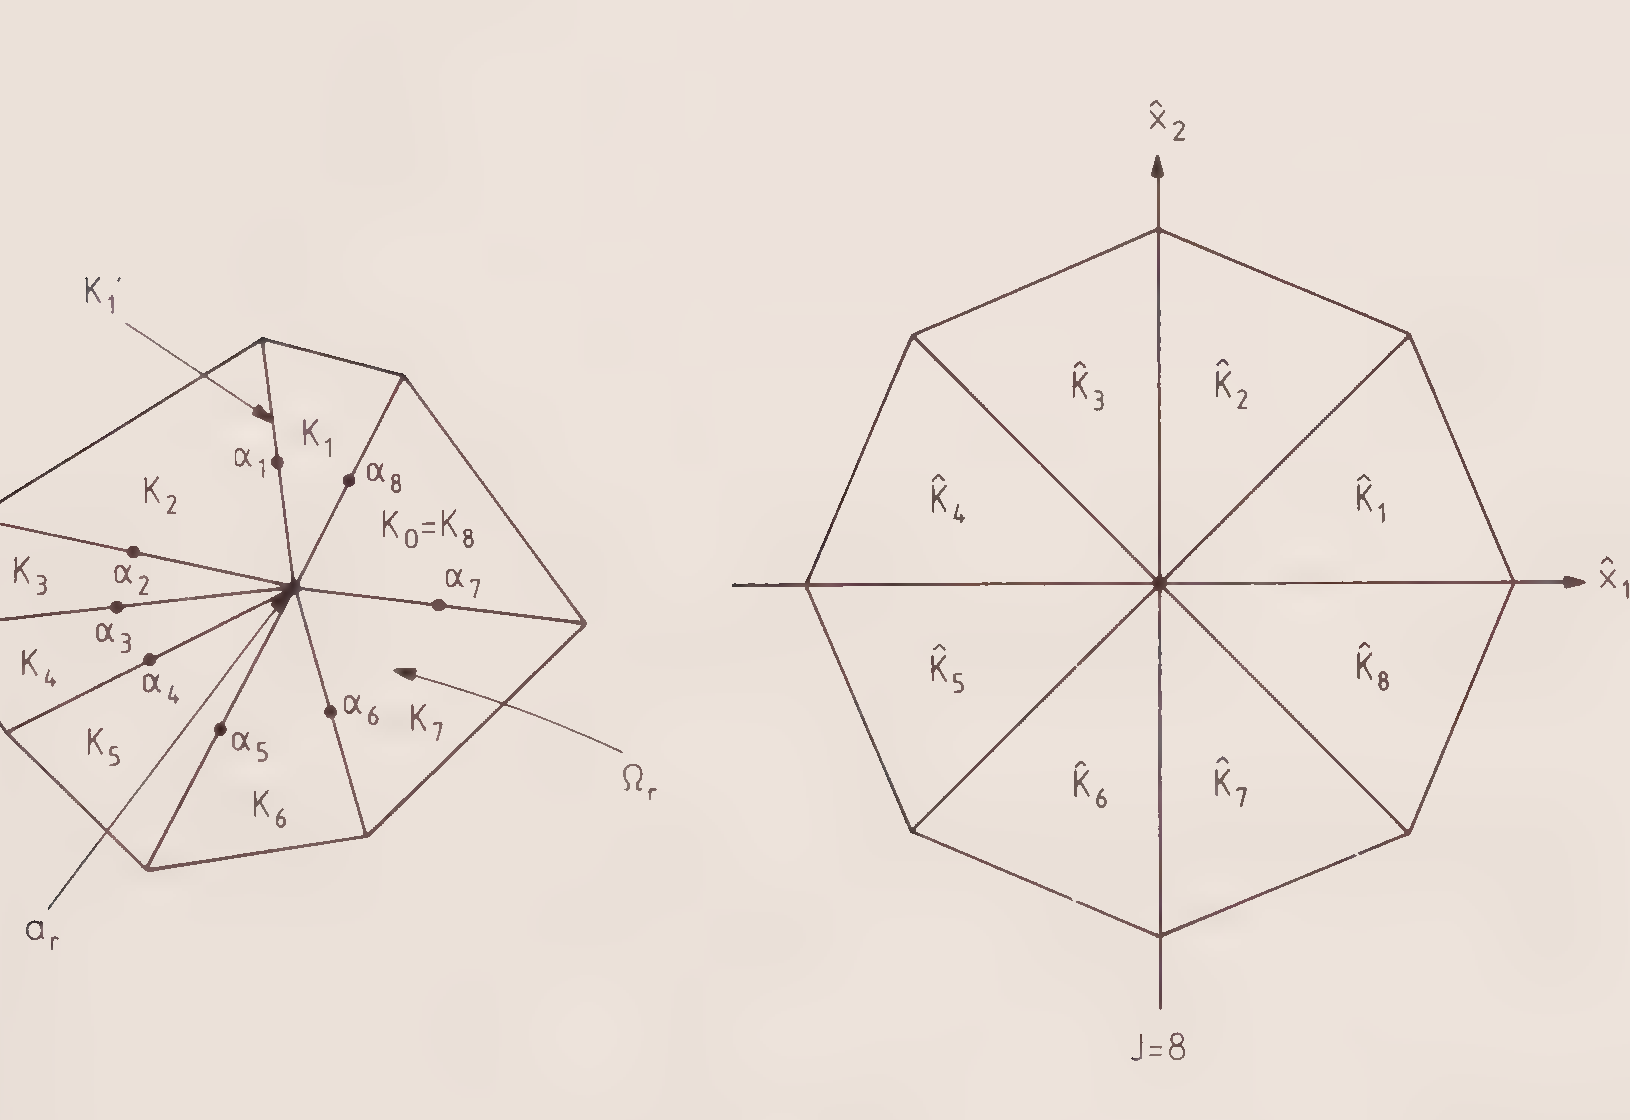
\includegraphics[width=.88\linewidth]{figures/chapter-02-figure-18.png}
\caption{一个宏单元及其参考宏单元.}
\label{fig:primitive-hood-taylor-macroelement}
\end{figure}

若这一假设成立, $\mathcal T_h$ 的每个单元 $\kappa$ 恰属于一个宏单元
$\Omega_r$. 此外, 所有节点 $a_r$ 都位于 $\Omega$ 内部这一事实意味着,
每个单元 $\kappa$ 恰有一条边位于其宏单元 $\Omega_r$ 的边界上, 并且至多
有一条边位于 $\Omega$ 的边界 $\Gamma$ 上.

实际中, 构造满足 \eqref{eq:primitive-hood-taylor-macroelement-partition}
的三角剖分并不困难. 通常先从粗网格出发, 再通过增加内部节点逐步细化.

回忆 \eqref{eq:primitive-local-spaces} 定义的空间:
\MathBookSourcePage{192}
\begin{equation}\label{eq:primitive-hood-taylor-local-spaces}
\left\{
\begin{aligned}
X_h(\Omega_r)&=\{\mathbf v_h\in X_h;
\ \operatorname{supp}(\mathbf v_h)\subset\Omega_r\},\\
Q_h(\Omega_r)&=\{q|_{\Omega_r};\ q\in Q_h\},\\
M_h(\Omega_r)&=Q_h(\Omega_r)\cap L_0^2(\Omega_r).
\end{aligned}
\right.
\end{equation}
我们来证明空间对 $(X_h(\Omega_r),M_h(\Omega_r))$ 满足局部 inf-sup 条件.

\setcounter{statement}{1}
\renewcommand{\theHstatement}{theorem.\thesection.\arabic{statement}}
\begin{Theorem}\label{thm:primitive-hood-taylor-local-inf-sup}
假设 $\mathcal T_h$ 是 $\Omega$ 的正则三角剖分, 且满足
\eqref{eq:primitive-hood-taylor-macroelement-partition}. 则存在与 $h,r$ 无关的常数
$\lambda^*>0$, 使
\begin{equation}\label{eq:primitive-hood-taylor-local-inf-sup}
\sup_{\mathbf v\in X_h(\Omega_r)}
\frac{\int_{\Omega_r}q\operatorname{div}\mathbf v\,dx}
{|\mathbf v|_{1,\Omega_r}}
\geq\lambda^*\|q\|_{0,\Omega_r}
\qquad\forall q\in M_h(\Omega_r).
\end{equation}
\end{Theorem}

\begin{Proof}
设 $J$ 是 $\Omega_r$ 中单元 $\kappa$ 的个数. 用从 $0$ 到 $J$ 的指标为它们
编号, 使 $\kappa_i$ 与 $\kappa_{i-1}$ 和 $\kappa_{i+1}$ 相邻, 且
$\kappa_0=\kappa_J$(如 Figure~\ref{fig:primitive-hood-taylor-macroelement}):
\[
\Omega_r=\bigcup_{i=1}^J\kappa_i.
\]
记 $\kappa_i'$ 为 $\kappa_i$ 与 $\kappa_{i+1}$ 的公共边, $\alpha_i$ 为
$\kappa_i'$ 的中点, $a_r$ 为 $\Omega_r$ 中所有 $\kappa_i$ 的公共顶点.

与 Section~\ref{sec:appendix-interpolation-discontinuous-functions} 一样,
通过连续分片仿射函数 $F_r$ 把 $\Omega_r$ 与参考集合
\[
\widehat\Omega=\bigcup_{i=1}^J\widehat\kappa_i
\quad\text{(参见 Figure~\ref{fig:primitive-hood-taylor-macroelement})}
\]
联系起来, 其中
\[
F_r(\widehat\kappa_i)=\kappa_i,
\qquad F_r(\widehat x)=B_i\widehat x+b_i
\quad\forall\widehat x\in\widehat\kappa_i.
\]
由于三角剖分正则, $J$ 由一个与 $r$ 无关的固定常数 $I$ 从上方控制,
因而至多有 $I$ 种不同的参考集合 $\widehat\Omega$. 这意味着与
$\widehat\Omega$ 和 $\widehat\kappa_i$ 有关的全部几何常数均可由与 $h,r$
无关的常数控制.

任取 $q_h\in Q_h(\Omega_r)$, 并取满足 $\mathbf v_h(a_r)=\mathbf0$ 的
$\mathbf v_h\in X_h(\Omega_r)$. 因为 $\mathbf v_h$ 在
$\partial\Omega_r$ 上消失且 $q_h\in H^1(\Omega_r)$, 有
\[
\int_{\Omega_r}\operatorname{div}\mathbf v_hq_h\,dx
=-\sum_{i=1}^J\int_{\kappa_i}
\mathbf v_h\cdot\operatorname{grad}q_h\,dx.
\]
$\mathbf v_h$ 的每个分量 $v$ 在 $\kappa_i$ 上均为 $P_2$ 多项式, 并在
$\kappa_i$ 的顶点处消失. 因而有求积公式
\[
\int_{\kappa_i}v\,dx
=\operatorname{meas}(\kappa_i)\frac13
\{v(\alpha_i)+v(\alpha_{i-1})\}.
\]
由于 $\operatorname{grad}q_h$ 在每个 $\kappa_i$ 上为常向量
(记 $\operatorname{grad}q_h|_{\kappa_i}=\mathbf g_i$), 该公式给出
\begin{equation}\label{eq:primitive-hood-taylor-local-quadrature}
\int_{\Omega_r}\operatorname{div}\mathbf v_hq_h\,dx
=-\frac13\sum_{i=1}^J\operatorname{meas}(\kappa_i)
\{\mathbf v(\alpha_i)+\mathbf v(\alpha_{i-1})\}\cdot\mathbf g_i.
\end{equation}

\MathBookSourcePage{193}
其次, 注意 $\partial q_h/\partial\tau$ 在单元界面处连续. 因此取
\[
\mathbf v(\alpha_i)=-(\mathbf g_i\cdot\mathbf t_i)\mathbf t_i
=-(\mathbf g_{i+1}\cdot\mathbf t_i)\mathbf t_i,
\]
其中 $\mathbf t_i$ 是 $\kappa_i'$ 的切向量, 长度为 $|\kappa_i'|$, 并且
(例如)指向 $\Omega_r$ 外部. 由此得到
\[
\int_{\Omega_r}\operatorname{div}\mathbf v_hq_h\,dx
=\frac13\sum_{i=1}^J\operatorname{meas}(\kappa_i)
\{(\mathbf g_i\cdot\mathbf t_i)^2+(\mathbf g_i\cdot\mathbf t_{i-1})^2\}.
\]
但根据 \eqref{eq:appendix-gradient-transform}, $\mathbf g\cdot\mathbf t$
在仿射变换下保持不变. 因而用显然的记号可写成
\[
\int_{\Omega_r}\operatorname{div}\mathbf v_hq_h\,dx
=\frac13\sum_{i=1}^J\operatorname{meas}(\kappa_i)
\{(\widehat{\mathbf g}_i\cdot\widehat{\mathbf t}_i)^2
+(\widehat{\mathbf g}_i\cdot\widehat{\mathbf t}_{i-1})^2\}.
\]
显然, 每组向量 $\{\widehat{\mathbf t}_{i-1},\widehat{\mathbf t}_i\}$
都是参考空间的一组基. 因而映射
$\widehat{\mathbf g}\mapsto
\{(\widehat{\mathbf g}\cdot\widehat{\mathbf t}_{i-1})^2
+(\widehat{\mathbf g}\cdot\widehat{\mathbf t}_i)^2\}^{1/2}$
等价于参考空间上的 Euclidean 范数. 再由
\[
|\widehat q|_{1,\widehat\kappa_i}^2
=\operatorname{meas}(\widehat\kappa_i)
\|\widehat{\mathbf g}_i\|^2,
\]
存在常数 $\widehat C_1>0$ 使
\begin{equation}\label{eq:primitive-hood-taylor-local-positive-form}
\int_{\Omega_r}\operatorname{div}\mathbf v_hq_h\,dx
\geq\widehat C_1\sum_{i=1}^J
\operatorname{meas}(\kappa_i)|\widehat q|_{1,\widehat\kappa_i}^2.
\end{equation}

另一方面, $\mathbf v_h$ 的定义给出
\begin{equation}\label{eq:primitive-hood-taylor-local-l2-bound}
\begin{aligned}
\|\mathbf v_h\|_{0,\kappa_i}^2
&\leq\widehat C_2\operatorname{meas}(\kappa_i)
\{\|\mathbf v(\alpha_{i-1})\|^2+\|\mathbf v(\alpha_i)\|^2\}\\
&\leq\widehat C_3\operatorname{meas}(\kappa_i)
[h_{\kappa_i}|\widehat q|_{1,\widehat\kappa_i}]^2.
\end{aligned}
\end{equation}
另一方面, Lemma~\ref{lem:appendix-local-inverse-inequality} 的论证给出
\begin{equation}\label{eq:primitive-hood-taylor-local-h1-bound}
\begin{aligned}
|\mathbf v_h|_{1,\kappa_i}^2
&\leq\widehat C_4
[\|B_i^{-1}\|\,\|\mathbf v_h\|_{0,\kappa_i}]^2\\
&\leq\widehat C_5\operatorname{meas}(\kappa_i)
[\sigma_{\kappa_i}|\widehat q|_{1,\widehat\kappa_i}]^2,
\end{aligned}
\end{equation}
其中第二式由 \eqref{eq:appendix-simplex-matrix-bounds} 和
\eqref{eq:primitive-hood-taylor-local-l2-bound} 得到. 因此, 由
\eqref{eq:primitive-hood-taylor-local-positive-form},
\eqref{eq:primitive-hood-taylor-local-h1-bound} 以及 $\mathcal T_h$ 的正则性,
\begin{equation}\label{eq:primitive-hood-taylor-local-preliminary-inf-sup}
\int_{\Omega_r}\operatorname{div}\mathbf v_hq_h\,dx
\geq\widehat C_6\sigma^{-1}|\mathbf v_h|_{1,\Omega_r}
\left\{\sum_{i=1}^J\operatorname{meas}(\kappa_i)
|\widehat q|_{1,\widehat\kappa_i}^2\right\}^{1/2}.
\end{equation}
还需证明, 对正则三角剖分有
\[
\left\{\sum_{i=1}^J\operatorname{meas}(\kappa_i)
|\widehat q|_{1,\widehat\kappa_i}^2\right\}^{1/2}
\geq\widehat C\|q\|_{0,\Omega_r}
\qquad\forall q\in H^1(\Omega_r)\cap L_0^2(\Omega_r).
\]
相应证明是 Lemma~\ref{lem:primitive-simplex-scaled-poincare} 证明的简单变体.
首先注意, 与 $F_r$ 复合把 $H^1(\Omega_r)$ 映入
$H^1(\widehat\Omega)$, 但不保持零均值. 这一小困难可通过把
